% answers.tex —— 1988 年·全国卷·理科 · 参考答案与详细解析片段
% 由 tools/generate_projects.py 依来源总账自 1988/1988_数学真题_全国理_试题.md + 1988/1988_数学真题_全国理_解析正文.md + 1988/1988_数学真题_全国理_答案要点.md 生成，勿手改（改源 MD 后重跑）


\begin{gktip}
固定源只有一页题面，没有答案和解析页。以下各题结论均为本库独立复算；第 9、19、22 题的图形依据固定源重绘。
\end{gktip}

\begin{answer}
\gksolhead{1}{}

\textbf{题目}：

\Needspace{5\baselineskip}
复数

\nopagebreak[4]
\[
\left(\frac{1-i}{1+i}\right)^2
\]

的值等于\mbox{（　　）}

（A）$1$　　（B）$-1$　　（C）$i$　　（D）$-i$

\Needspace{4\baselineskip}
\textbf{解析}

\Needspace{5\baselineskip}
有

\nopagebreak[4]
\[
\frac{1-i}{1+i}
=\frac{(1-i)^2}{(1+i)(1-i)}
=-i.
\]

所以原式为 $(-i)^2=-1$，答案为 B。

\gkanswer{答案：B}

\end{answer}
\begin{answer}
\gksolhead{2}{}

\textbf{题目}：

\Needspace{5\baselineskip}
设圆 $M$ 的方程为

\nopagebreak[4]
\[
(x-3)^2+(y-2)^2=2,
\]

\Needspace{5\baselineskip}
直线 $L$ 的方程为

\nopagebreak[4]
\[
x+y-3=0,
\]

点 $P$ 的坐标为 $(2,1)$，那么\mbox{（　　）}

（A）点 $P$ 在直线 $L$ 上，但不在圆 $M$ 上

（B）点 $P$ 在圆 $M$ 上，但不在直线 $L$ 上

（C）点 $P$ 既在圆 $M$ 上，又在直线 $L$ 上

（D）点 $P$ 既不在直线 $L$ 上，也不在圆 $M$ 上

\Needspace{4\baselineskip}
\textbf{解析}

\Needspace{5\baselineskip}
点 $P=(2,1)$ 满足 $x+y-3=0$。同时

\nopagebreak[4]
\[
(2-3)^2+(1-2)^2=2,
\]

满足圆的方程。因此点 $P$ 同时在圆 $M$ 和直线 $L$ 上，答案为 C。

\gkanswer{答案：C}

\end{answer}
\begin{answer}
\gksolhead{3}{}

\textbf{题目}：

集合 $\{1,2,3\}$ 的子集共有\mbox{（　　）}

（A）7 个　　（B）8 个　　（C）6 个　　（D）5 个

\Needspace{4\baselineskip}
\textbf{解析}

\Needspace{5\baselineskip}
含有 $3$ 个元素的集合共有

\nopagebreak[4]
\[
2^3=8
\]

个子集，答案为 B。

\gkanswer{答案：B}

\end{answer}
\begin{answer}
\gksolhead{4}{}

\textbf{题目}：

\Needspace{5\baselineskip}
已知双曲线方程

\nopagebreak[4]
\[
\frac{x^2}{20}-\frac{y^2}{5}=1,
\]

那么它的焦距是\mbox{（　　）}

（A）$10$　　（B）$5$　　（C）$\sqrt{15}$　　（D）$2\sqrt{15}$

\Needspace{4\baselineskip}
\textbf{解析}

\Needspace{5\baselineskip}
双曲线的参数满足

\nopagebreak[4]
\[
c^2=a^2+b^2=20+5=25,
\qquad c=5.
\]

焦距为 $2c=10$，答案为 A。

\gkanswer{答案：A}

\end{answer}
\begin{answer}
\gksolhead{5}{}

\textbf{题目}：

\Needspace{5\baselineskip}
在

\nopagebreak[4]
\[
(x-\sqrt3)^{10}
\]

的展开式中，$x^6$ 的系数是\mbox{（　　）}

（A）$-27C_{10}^{6}$　　（B）$27C_{10}^{4}$

（C）$-9C_{10}^{6}$　　（D）$9C_{10}^{4}$

\Needspace{4\baselineskip}
\textbf{解析}

\Needspace{5\baselineskip}
要得到 $x^6$ 项，需从

\nopagebreak[4]
\[
\binom{10}{4}x^6(-\sqrt3)^4
\]

\Needspace{5\baselineskip}
取项。因此系数为

\nopagebreak[4]
\[
9\binom{10}{4},
\]

答案为 D。

\gkanswer{答案：D}

\end{answer}
\begin{answer}
\gksolhead{6}{}

\textbf{题目}：

\Needspace{5\baselineskip}
函数

\nopagebreak[4]
\[
y=\cos^4x-\sin^4x
\]

的最小正周期是\mbox{（　　）}

（A）$\pi$　　（B）$2\pi$　　（C）$\dfrac\pi2$　　（D）$4\pi$

\Needspace{4\baselineskip}
\textbf{解析}

\Needspace{5\baselineskip}
利用平方差：

\nopagebreak[4]
\[
\cos^4x-\sin^4x
=(\cos^2x-\sin^2x)(\cos^2x+\sin^2x)
=\cos2x.
\]

其最小正周期为 $\pi$，答案为 A。

\gkanswer{答案：A}

\end{answer}
\begin{answer}
\gksolhead{7}{}

\textbf{题目}：

\Needspace{5\baselineskip}
方程

\nopagebreak[4]
\[
4\cos^2x-4\sqrt3\cos x+3=0
\]

的解集是\mbox{（　　）}

（A）$\left\{x\mid x=k\pi+(-1)^k\frac\pi6,\ k\in\mathbb Z\right\}$

（B）$\left\{x\mid x=k\pi+(-1)^k\frac\pi3,\ k\in\mathbb Z\right\}$

（C）$\left\{x\mid x=2k\pi\pm\frac\pi6,\ k\in\mathbb Z\right\}$

（D）$\left\{x\mid x=2k\pi\pm\frac\pi3,\ k\in\mathbb Z\right\}$

\Needspace{4\baselineskip}
\textbf{解析}

\Needspace{5\baselineskip}
原方程为

\nopagebreak[4]
\[
(2\cos x-\sqrt3)^2=0,
\]

\Needspace{5\baselineskip}
所以 $\cos x=\sqrt3/2$，解集为

\nopagebreak[4]
\[
x=2k\pi\pm\frac\pi6,\qquad k\in\mathbb Z.
\]

答案为 C。

\gkanswer{答案：C}

\end{answer}
\begin{answer}
\gksolhead{8}{}

\textbf{题目}：

\Needspace{5\baselineskip}
极坐标方程

\nopagebreak[4]
\[
\rho=\frac4{3-2\cos\theta}
\]

所表示的曲线是\mbox{（　　）}

（A）圆　　（B）双曲线右支　　（C）抛物线　　（D）椭圆

\Needspace{4\baselineskip}
\textbf{解析}

\Needspace{5\baselineskip}
极坐标方程化为

\nopagebreak[4]
\[
\rho(3-2\cos\theta)=4,
\qquad
3\rho=4+2x.
\]

\Needspace{5\baselineskip}
平方并用 $\rho^2=x^2+y^2$，得

\nopagebreak[4]
\[
9(x^2+y^2)=(4+2x)^2,
\]

\Needspace{5\baselineskip}
即

\nopagebreak[4]
\[
5x^2+9y^2-16x-16=0.
\]

这是椭圆，答案为 D。

\gkanswer{答案：D}

\end{answer}
\begin{answer}
\gksolhead{9}{}

\textbf{题目}：

如图，正四棱台中，$A'D'$ 所在的直线与 $BB'$ 所在的直线是\mbox{（　　）}
\nopagebreak[4]
\begin{center}% 1988 年全国卷理科第 9 题：正四棱台
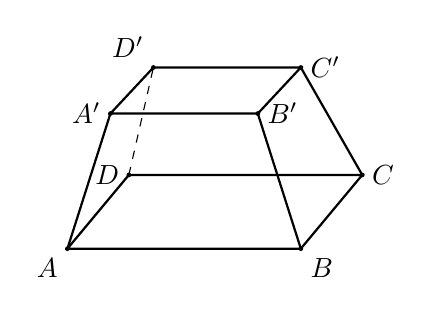
\begin{tikzpicture}[scale=0.78,>=stealth]
  \coordinate (A) at (0,0);
  \coordinate (B) at (3.8,0);
  \coordinate (C) at (4.8,1.2);
  \coordinate (D) at (1.0,1.2);
  \coordinate (Ap) at (0.7,2.2);
  \coordinate (Bp) at (3.1,2.2);
  \coordinate (Cp) at (3.8,2.95);
  \coordinate (Dp) at (1.4,2.95);
  \draw[thick] (A)--(B)--(C)--(D)--cycle;
  \draw[thick] (Ap)--(Bp)--(Cp)--(Dp)--cycle;
  \draw[thick] (A)--(Ap) (B)--(Bp) (C)--(Cp);
  \draw[dashed] (D)--(Dp);
  \fill (A) circle (1.1pt) node[below left] {$A$};
  \fill (B) circle (1.1pt) node[below right] {$B$};
  \fill (C) circle (1.1pt) node[right] {$C$};
  \fill (D) circle (1.1pt) node[left] {$D$};
  \fill (Ap) circle (1.1pt) node[left] {$A'$};
  \fill (Bp) circle (1.1pt) node[right] {$B'$};
  \fill (Cp) circle (1.1pt) node[right] {$C'$};
  \fill (Dp) circle (1.1pt) node[above left] {$D'$};
\end{tikzpicture}
\end{center}
\nopagebreak[4]
（A）相交直线　　（B）平行直线

（C）不互相垂直的异面直线　　（D）互相垂直的异面直线

\Needspace{4\baselineskip}
\textbf{解析}

在正四棱台中，$A'D'$ 平行于底面边 $AD$，而 $BB'$ 为侧棱。两直线不相交且不平行。

若它们互相垂直，则过 $B'$ 作的平行于 $AD$ 的直线也应与 $BB'$ 垂直；但正四棱台的侧棱方向与顶面边方向一般不满足这一关系。由图形的空间位置可知二者为不互相垂直的异面直线，答案为 C。

\gkanswer{答案：C}

\end{answer}
\begin{answer}
\gksolhead{10}{}

\Needspace{5\baselineskip}
\textbf{题目}：

\nopagebreak[4]
\[
\tan\left(\arctan\frac15+\arctan3\right)
\]

的值等于\mbox{（　　）}

（A）$4$　　（B）$\dfrac12$　　（C）$\dfrac18$　　（D）$8$

\Needspace{4\baselineskip}
\textbf{解析}

\Needspace{5\baselineskip}
由正切加法公式

\nopagebreak[4]
\[
\tan\left(\arctan\frac15+\arctan3\right)
=\frac{\frac15+3}{1-\frac35}
=\frac{\frac{16}{5}}{\frac25}=8.
\]

答案为 D。

\gkanswer{答案：D}

\end{answer}
\begin{answer}
\gksolhead{11}{}

\textbf{题目}：

设命题甲：$\triangle ABC$ 的一个内角为 $60^\circ$；命题乙：$\triangle ABC$ 的三内角的度数成等差数列。那么\mbox{（　　）}

（A）甲是乙的充分条件，但不是必要条件

（B）甲是乙的必要条件，但不是充分条件

（C）甲是乙的充要条件

（D）甲不是乙的充分条件，也不是乙的必要条件

\Needspace{4\baselineskip}
\textbf{解析}

\Needspace{5\baselineskip}
三角形内角成等差数列时，中间的内角为

\nopagebreak[4]
\[
\frac{180^\circ}{3}=60^\circ.
\]

因此乙是甲的充分条件。反过来，一个内角为 $60^\circ$ 并不能保证另外两个角关于它对称，例如角度可为 $60^\circ,50^\circ,70^\circ$。所以乙不是甲的充分条件，甲是乙的必要但非充分条件，答案为 B。

\gkanswer{答案：B}

\end{answer}
\begin{answer}
\gksolhead{12}{}

\textbf{题目}：

\Needspace{5\baselineskip}
在复平面内，若复数 $z$ 满足

\nopagebreak[4]
\[
|z+1|=|z-i|,
\]

则 $z$ 所对应的点 $Z$ 的集合构成的图形是\mbox{（　　）}

（A）圆　　（B）直线　　（C）椭圆　　（D）双曲线

\Needspace{4\baselineskip}
\textbf{解析}

\Needspace{5\baselineskip}
设 $z=x+iy$。由

\nopagebreak[4]
\[
|z+1|=|z-i|
\]

\Needspace{5\baselineskip}
得

\nopagebreak[4]
\[
(x+1)^2+y^2=x^2+(y-1)^2,
\]

\Needspace{5\baselineskip}
即

\nopagebreak[4]
\[
x+y=0.
\]

这是直线，答案为 B。

\gkanswer{答案：B}

\end{answer}
\begin{answer}
\gksolhead{13}{}

\textbf{题目}：

\Needspace{5\baselineskip}
如果曲线

\nopagebreak[4]
\[
x^2-y^2-2x-2y-1=0
\]

\Needspace{5\baselineskip}
经过平移坐标轴后的新方程为

\nopagebreak[4]
\[
x'^2-y'^2=1,
\]

那么新坐标系的原点在原坐标系中的坐标为\mbox{（　　）}

（A）$(1,1)$　　（B）$(-1,-1)$　　（C）$(-1,1)$　　（D）$(1,-1)$

\Needspace{4\baselineskip}
\textbf{解析}

\Needspace{5\baselineskip}
原方程配方为

\nopagebreak[4]
\[
(x-1)^2-(y+1)^2=1.
\]

平移后的新原点在原坐标系中为 $(1,-1)$，答案为 D。

\gkanswer{答案：D}

\end{answer}
\begin{answer}
\gksolhead{14}{}

\textbf{题目}：

假设在 200 件产品中有 3 件次品，现在从中任意抽取 5 件，其中至少有 2 件次品的抽法有\mbox{（　　）}

（A）$C_3^2C_{197}^3$ 种

（B）$C_3^2C_{197}^3+C_3^3C_{197}^2$ 种

（C）$C_{200}^5-C_{197}^5$ 种

（D）$C_{200}^5-C_3^1C_{197}^4$ 种

\Needspace{4\baselineskip}
\textbf{解析}

\Needspace{5\baselineskip}
至少抽到两件次品有两种互斥情形：

\nopagebreak[4]
\[
C_3^2C_{197}^3+C_3^3C_{197}^2.
\]

答案为 B。

\gkanswer{答案：B}

\end{answer}
\begin{answer}
\gksolhead{15}{}

\textbf{题目}：

已知二面角 $\alpha-AB-\beta$ 的平面角是锐角，$C$ 是平面 $\alpha$ 内一点（它不在棱 $AB$ 上），点 $D$ 是点 $C$ 在面 $\beta$ 上的投影，点 $E$ 是棱 $AB$ 上满足 $\angle CEB$ 为锐角的任一点，那么\mbox{（　　）}

（A）$\angle CEB>\angle DEB$

（B）$\angle CEB=\angle DEB$

（C）$\angle CEB<\angle DEB$

（D）$\angle CEB$ 与 $\angle DEB$ 的大小关系不能确定

\Needspace{4\baselineskip}
\textbf{解析}

\Needspace{5\baselineskip}
以棱 $AB$ 为 $x$ 轴建立局部坐标。设 $C$ 在平面 $\alpha$ 内到棱的垂距为 $h$，二面角为锐角 $\theta$。正交投影到平面 $\beta$ 后，平行于棱的分量不变，而垂直于棱的分量变为 $h\cos\theta$。

\nopagebreak[4]
\[
\tan\angle CEB=\frac{h}{|EB|},
\qquad
\tan\angle DEB=\frac{h\cos\theta}{|EB|}.
\]

\Needspace{5\baselineskip}
因为 $0<\cos\theta<1$ 且 $\angle CEB$ 为锐角，所以

\nopagebreak[4]
\[
\angle DEB<\angle CEB.
\]

故答案为 A。

\gkanswer{答案：A}

\end{answer}
\begin{answer}
\gksolhead{16}{}

\textbf{题目}：

\Needspace{5\baselineskip}
求复数

\nopagebreak[4]
\[
\sqrt3-i
\]

的模和辐角的主值。

\Needspace{4\baselineskip}
\textbf{解析}

\Needspace{5\baselineskip}
复数 $\sqrt3-i$ 的模为

\nopagebreak[4]
\[
\sqrt{3+1}=2.
\]

\Needspace{5\baselineskip}
它位于第四象限，辐角主值为

\nopagebreak[4]
\[
-\arctan\frac1{\sqrt3}=-\frac\pi6.
\]

\gkanswer{答案：模为 $2$，辐角主值为 $-\dfrac\pi6$}

\end{answer}
\begin{answer}
\gksolhead{17}{}

\textbf{题目}：

\Needspace{5\baselineskip}
解方程

\nopagebreak[4]
\[
9^{-x}-2\cdot3^{1-x}=27.
\]

\Needspace{4\baselineskip}
\textbf{解析}

\Needspace{5\baselineskip}
令 $u=3^{-x}>0$，则 $9^{-x}=u^2$ 且 $3^{1-x}=3u$，方程化为

\nopagebreak[4]
\[
u^2-6u-27=0.
\]

所以 $(u-9)(u+3)=0$。取正根 $u=9$，得到 $3^{-x}=3^2$，故 $x=-2$。

\gkanswer{答案：$x=-2$}

\end{answer}
\begin{answer}
\gksolhead{18}{}

\textbf{题目}：

\Needspace{5\baselineskip}
已知

\nopagebreak[4]
\[
\sin\theta=-\frac35,\qquad
3\pi<\theta<\frac{7\pi}{2},
\]

\Needspace{5\baselineskip}
求

\nopagebreak[4]
\[
\tan\frac\theta2.
\]

\Needspace{4\baselineskip}
\textbf{解析}

\Needspace{5\baselineskip}
由 $3\pi<\theta<7\pi/2$ 可知 $\theta$ 的终边在第三象限，所以

\nopagebreak[4]
\[
\cos\theta=-\frac45.
\]

\Needspace{5\baselineskip}
半角公式给出

\nopagebreak[4]
\[
\tan\frac\theta2
=\frac{\sin\theta}{1+\cos\theta}
=\frac{-3/5}{1-4/5}=-3.
\]

\gkanswer{答案：$\tan\dfrac\theta2=-3$}

\end{answer}
\begin{answer}
\gksolhead{19}{}

\textbf{题目}：

\Needspace{5\baselineskip}
如图，四棱锥 $S-ABCD$ 的底面是边长为 $1$ 的正方形，侧棱 $SB$ 垂直于底面，并且

\nopagebreak[4]
\[
SB=\sqrt3.
\]

用 $\alpha$ 表示 $\angle ASD$，求 $\sin\alpha$。
\nopagebreak[4]
\begin{center}% 1988 年全国卷理科第 19 题：四棱锥
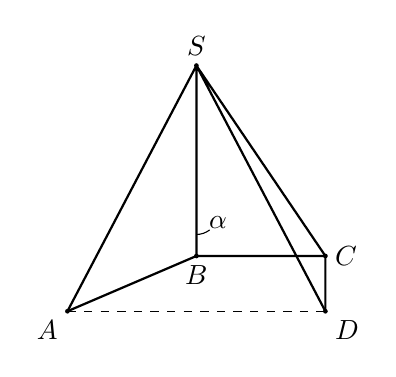
\begin{tikzpicture}[scale=0.78,>=stealth]
  \coordinate (S) at (2.1,4.0);
  \coordinate (B) at (2.1,0.9);
  \coordinate (A) at (0,0);
  \coordinate (C) at (4.2,0.9);
  \coordinate (D) at (4.2,0);
  \draw[thick] (S)--(A) (S)--(B) (S)--(C) (S)--(D);
  \draw[thick] (A)--(B)--(C)--(D);
  \draw[dashed] (A)--(D) (S)--(B);
  \draw (2.1,1.25) arc (-90:-52:0.35);
  \node at (2.45,1.45) {$\alpha$};
  \fill (S) circle (1.1pt) node[above] {$S$};
  \fill (A) circle (1.1pt) node[below left] {$A$};
  \fill (B) circle (1.1pt) node[below] {$B$};
  \fill (C) circle (1.1pt) node[right] {$C$};
  \fill (D) circle (1.1pt) node[below right] {$D$};
\end{tikzpicture}
\end{center}
\nopagebreak[4]
\Needspace{4\baselineskip}
\textbf{解析}

\Needspace{5\baselineskip}
设正方形底面为 $ABCD$，取

\nopagebreak[4]
\[
B=(0,0,0),\quad A=(1,0,0),\quad
C=(0,1,0),\quad D=(1,1,0),\quad
S=(0,0,\sqrt3).
\]

\Needspace{5\baselineskip}
则

\nopagebreak[4]
\[
\overrightarrow{SA}=(1,0,-\sqrt3),
\qquad
\overrightarrow{SD}=(1,1,-\sqrt3).
\]

\Needspace{5\baselineskip}
由向量夹角公式

\nopagebreak[4]
\[
\cos\alpha
=\frac{\overrightarrow{SA}\cdot\overrightarrow{SD}}
{|\overrightarrow{SA}||\overrightarrow{SD}|}
=\frac4{2\sqrt5}=\frac2{\sqrt5}.
\]

\Needspace{5\baselineskip}
所以

\nopagebreak[4]
\[
\sin\alpha=\frac1{\sqrt5}.
\]

\gkanswer{答案：$\sin\alpha=\dfrac1{\sqrt5}$}

\end{answer}
\begin{answer}
\gksolhead{20}{}

\textbf{题目}：

\Needspace{5\baselineskip}
已知等比数列 $\{a_n\}$ 的公比 $q>1$，并且 $a_1=b$（$b\ne0$）。求

\nopagebreak[4]
\[
\lim_{n\to\infty}
\frac{a_1+a_2+a_3+\cdots+a_n}
{a_6+a_7+a_8+\cdots+a_n}.
\]

\Needspace{4\baselineskip}
\textbf{解析}

\Needspace{5\baselineskip}
由等比数列

\nopagebreak[4]
\[
a_k=bq^{k-1}.
\]

\Needspace{5\baselineskip}
分子和为

\nopagebreak[4]
\[
b\frac{q^n-1}{q-1},
\]

\Needspace{5\baselineskip}
分母和为

\nopagebreak[4]
\[
bq^5\frac{q^{n-5}-1}{q-1}.
\]

\Needspace{5\baselineskip}
当 $q>1$ 且 $n\to\infty$ 时，最高次项决定比值，故

\nopagebreak[4]
\[
\lim_{n\to\infty}
\frac{a_1+\cdots+a_n}{a_6+\cdots+a_n}
=\frac1{q^5}.
\]

\gkanswer{答案：$\dfrac1{q^5}$}

\end{answer}
\begin{answer}
\gksolhead{21}{}

\textbf{题目}：

\Needspace{5\baselineskip}
已知 $\tan x=a$，求

\nopagebreak[4]
\[
\frac{3\sin x+\sin3x}{3\cos x+\cos3x}
\]

的值。

\Needspace{4\baselineskip}
\textbf{解析}

\Needspace{5\baselineskip}
令 $s=\sin x,c=\cos x$，则

\nopagebreak[4]
\[
3\sin x+\sin3x
=3s+3s-4s^3
=2s(1+2c^2),
\]

\Needspace{5\baselineskip}
而

\nopagebreak[4]
\[
3\cos x+\cos3x
=3c+4c^3-3c=4c^3.
\]

\Needspace{5\baselineskip}
因此

\nopagebreak[4]
\[
\frac{3\sin x+\sin3x}{3\cos x+\cos3x}
=\frac{s(1+2c^2)}{2c^3}.
\]

\Needspace{5\baselineskip}
用 $a=\tan x=s/c$ 和 $c^2=1/(1+a^2)$ 化简得

\nopagebreak[4]
\[
\frac{a(a^2+3)}2.
\]

\gkanswer{答案：$\dfrac{a(a^2+3)}2$}

\end{answer}
\begin{answer}
\gksolhead{22}{}

\textbf{题目}：

如图，正三棱锥 $S-ABC$ 的侧面是边长为 $a$ 的正三角形，$D$ 是 $SA$ 的中点，$E$ 是 $BC$ 的中点，求 $\triangle SDE$ 绕直线 $SE$ 旋转一周所得的旋转体的体积。
\nopagebreak[4]
\begin{center}% 1988 年全国卷理科第 22 题：正三棱锥及中点
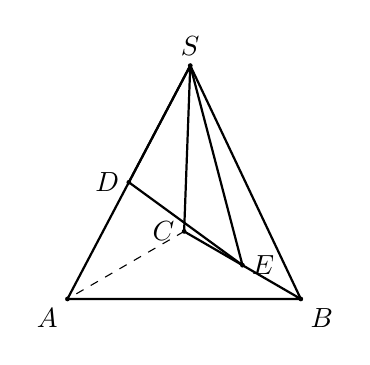
\begin{tikzpicture}[scale=0.78,>=stealth]
  \coordinate (S) at (2.0,3.8);
  \coordinate (A) at (0,0);
  \coordinate (B) at (3.8,0);
  \coordinate (C) at (1.9,1.1);
  \coordinate (D) at (1.0,1.9);
  \coordinate (E) at (2.85,0.55);
  \draw[thick] (S)--(A) (S)--(B) (S)--(C);
  \draw[thick] (A)--(B) (B)--(C);
  \draw[dashed] (C)--(A);
  \draw[thick] (S)--(E) (D)--(E) (S)--(D);
  \fill (S) circle (1.1pt) node[above] {$S$};
  \fill (A) circle (1.1pt) node[below left] {$A$};
  \fill (B) circle (1.1pt) node[below right] {$B$};
  \fill (C) circle (1.1pt) node[left] {$C$};
  \fill (D) circle (1.1pt) node[left] {$D$};
  \fill (E) circle (1.1pt) node[right] {$E$};
\end{tikzpicture}
\end{center}
\nopagebreak[4]
\Needspace{4\baselineskip}
\textbf{解析}

\Needspace{5\baselineskip}
正三棱锥且侧面为边长 $a$ 的正三角形时，它是正四面体。三角形 $SDE$ 的三边为

\nopagebreak[4]
\[
SD=\frac a2,\qquad
SE=\frac{\sqrt3}{2}a,\qquad
DE=\frac{a}{\sqrt2}.
\]

\Needspace{5\baselineskip}
由海伦公式或向量计算，三角形面积为

\nopagebreak[4]
\[
[SDE]=\frac{\sqrt2}{8}a^2.
\]

\Needspace{5\baselineskip}
其重心到旋转轴 $SE$ 的距离是三角形高 $a\sqrt6/6$ 的三分之一，即 $a\sqrt6/18$。由帕普斯定理，旋转体体积为

\nopagebreak[4]
\[
V=[SDE]\cdot2\pi\cdot\frac{a\sqrt6}{18}
=\frac{\sqrt3\pi a^3}{36}.
\]

\gkanswer{答案：$\dfrac{\sqrt3\pi a^3}{36}$}

\end{answer}
\begin{answer}
\gksolhead{23}{}

\textbf{题目}：

\Needspace{5\baselineskip}
设 $a>0$，$a\ne1$，$t>0$，比较

\nopagebreak[4]
\[
\frac12\log_a t
\qquad\text{\text{与}}\qquad
\log_a\frac{t+1}{2}
\]

的大小，并证明你的结论。

\Needspace{4\baselineskip}
\textbf{解析}

\Needspace{5\baselineskip}
因为

\nopagebreak[4]
\[
\frac12\log_a t=\log_a\sqrt t,
\]

\Needspace{5\baselineskip}
而算术平均数不小于几何平均数：

\nopagebreak[4]
\[
\sqrt t\le\frac{t+1}{2}.
\]

\Needspace{5\baselineskip}
当 $a>1$ 时对数函数递增，所以

\nopagebreak[4]
\[
\frac12\log_a t\le\log_a\frac{t+1}{2}.
\]

当 $0<a<1$ 时对数函数递减，不等号反向。$t=1$ 时取得等号。

\gkanswer{答案：若 $a>1$，则 $\dfrac12\log_a t\leq\log_a\dfrac{t+1}{2}$；若 $0<a<1$，不等号反向；$t=1$ 时等号成立。}

\end{answer}
\begin{answer}
\gksolhead{24}{}

\textbf{题目}：

\Needspace{5\baselineskip}
给定实数 $a$，且 $a\ne0,\ a\ne1$，设函数

\nopagebreak[4]
\[
y=\frac{x-1}{ax-1}
\qquad\left(x\in R,\ x\ne\frac1a\right).
\]

证明：

（1） 经过这个函数图象上任意两个不同的点的直线不平行于 $x$ 轴；

（2） 这个函数的图象关于直线 $y=x$ 成轴对称图形。

\Needspace{4\baselineskip}
\textbf{解析}

\gksubpart{（1）}

\Needspace{5\baselineskip}
设图象上两个不同点对应横坐标 $x_1\ne x_2$。若它们的纵坐标相等，则

\nopagebreak[4]
\[
\frac{x_1-1}{ax_1-1}
=\frac{x_2-1}{ax_2-1}.
\]

\Needspace{5\baselineskip}
交叉相乘后得到

\nopagebreak[4]
\[
(a-1)(x_1-x_2)=0,
\]

与 $a\ne1$ 及 $x_1\ne x_2$ 矛盾。因此任意两个不同点的连线不平行于 $x$ 轴。

\gksubpart{（2）}

\Needspace{5\baselineskip}
设

\nopagebreak[4]
\[
y=\frac{x-1}{ax-1}.
\]

\Needspace{5\baselineskip}
解出 $x$：

\nopagebreak[4]
\[
x=\frac{y-1}{ay-1}.
\]

这说明反函数的表达式与原函数相同，故函数图象关于 $y=x$ 成轴对称图形。

\gkanswer{答案（1）：经过图象上任意两个不同点的直线不平行于 $x$ 轴。}

\gkanswer{答案（2）：函数图象关于直线 $y=x$ 成轴对称图形。}

\end{answer}
\begin{answer}
\gksolhead{25}{}

\textbf{题目}：

\Needspace{5\baselineskip}
直线 $L$ 的方程为

\nopagebreak[4]
\[
x=-\frac p2,\qquad p>0;
\]

\Needspace{5\baselineskip}
椭圆的中心为

\nopagebreak[4]
\[
D\left(2+\frac p2,0\right),
\]

\Needspace{5\baselineskip}
焦点在 $x$ 轴上，长半轴长为 $2$，短半轴长为 $1$，它的一个顶点为

\nopagebreak[4]
\[
A\left(\frac p2,0\right).
\]

问 $p$ 在哪个范围内取值时，椭圆上有四个不同的点，它们中每一个点到点 $A$ 的距离等于该点到直线 $L$ 的距离。

\Needspace{4\baselineskip}
\textbf{解析}

\Needspace{5\baselineskip}
椭圆中心为 $D(2+p/2,0)$，长半轴为 $2$、短半轴为 $1$，且左顶点为

\nopagebreak[4]
\[
A\left(\frac p2,0\right).
\]

\Needspace{5\baselineskip}
对椭圆上的点 $(x,y)$，条件“到 $A$ 的距离等于到直线 $x=-p/2$ 的距离”平方后化为一条抛物线与椭圆的交点条件。将椭圆方程代入并考察交点关于 $x$ 轴成对出现，可得有四个不同交点的充要条件为

\nopagebreak[4]
\[
0<p<\frac13.
\]

\gkanswer{答案：$0<p<\dfrac13$}

\end{answer}